\documentclass[11pt,a4paper]{article}

\usepackage[a4paper,margin=1in]{geometry}
\usepackage[utf8]{inputenc}
\usepackage[T1]{fontenc}
\usepackage{lmodern}
\usepackage{microtype}
\usepackage{parskip}

\usepackage{amsmath}
\usepackage{amssymb}
\usepackage{mathtools}

\usepackage{graphicx}
\usepackage{caption}
\usepackage{subcaption}
\usepackage{float}

\usepackage{booktabs}
\usepackage{tabularx}
\usepackage{multirow}

\usepackage[table]{xcolor}
\definecolor{linkblue}{HTML}{1f6feb}
\definecolor{citegreen}{HTML}{2ca02c}
\definecolor{codebg}{HTML}{f6f8fa}
\definecolor{codecomment}{HTML}{6a737d}
\definecolor{codekey}{HTML}{d73a49}
\definecolor{codestr}{HTML}{032f62}
\definecolor{codenum}{HTML}{005cc5}

\usepackage[colorlinks=true,linkcolor=linkblue,citecolor=citegreen,urlcolor=linkblue]{hyperref}

\usepackage{listings}
\lstdefinestyle{pylike}{
  backgroundcolor=\color{codebg},
  basicstyle=\ttfamily\small,
  commentstyle=\color{codecomment}\itshape,
  keywordstyle=\color{codekey}\bfseries,
  stringstyle=\color{codestr},
  numberstyle=\color{codecomment}\tiny,
  showstringspaces=false,
  breaklines=true,
  numbers=left,
  numbersep=6pt,
  tabsize=4,
  language=Python,
  keepspaces=true,
  frame=single,
  rulecolor=\color{codecomment!30},
  aboveskip=8pt, belowskip=8pt,
}
\lstset{style=pylike}

\usepackage{authblk}
\usepackage{titlesec}
\titleformat{\section}{\Large\bfseries}{\thesection}{0.6em}{}
\titleformat{\subsection}{\large\bfseries}{\thesubsection}{0.6em}{}
\titlespacing*{\section}{0pt}{1.6ex plus 0.3ex minus 0.2ex}{0.8ex plus 0.2ex}
\titlespacing*{\subsection}{0pt}{1.2ex plus 0.2ex minus 0.2ex}{0.6ex plus 0.2ex}

\title{\textbf{Feedback-Augmented RT-DETR:} \\[0.2em] A Cross-Attention Refinement Strategy \\ for Enhanced Small-Object Detection}
\author[1]{Hatem Saadallah}
\author[1]{Nour Jennane}
\affil[1]{Computer Vision and Image Processing, Bocconi University}
\date{April 2026}

\begin{document}

\maketitle

\begin{abstract}
Real-time transformer detectors achieve strong overall accuracy but consistently underperform on small objects. We propose a \emph{decoder-to-encoder feedback} module that uses early decoder predictions to refine the encoder memory before later decoder layers attend over it. A direct implementation produced no measurable contribution at inference ($\Delta\mathrm{AP}_S = 0.00$); we trace the cause to the learnable gate decaying to near zero during training. Two purely structural fixes --- a \emph{gate floor} that prevents the gate from collapsing, and a \emph{level mask} restricting feedback to the P2 and P3 features where small objects live --- turn the mechanism into a causally measurable one, with $\Delta\mathrm{AP}_S = +0.99$ on COCO \textsc{val2017}. The fixes add zero new parameters.

\end{abstract}

\section{Introduction}
\label{sec:intro}

Object detection at real-time rates is dominated by two paradigms: NMS-based one-stage detectors (the YOLO family~\cite{redmon2016yolo,wang2023yolov7}) and end-to-end transformer detectors that learn a permutation-invariant set prediction (DETR~\cite{carion2020detr} and its descendants~\cite{zhu2021deformable,liu2022dabdetr,zhang2023dino}). RT-DETR~\cite{lyu2024rtdetr} closed the speed gap between these paradigms by introducing a hybrid encoder that decouples intra-scale interaction (Attention-based In-scale Feature Interaction, AIFI) from cross-scale fusion (CNN-based Cross-scale Feature Fusion, CCFF), and demonstrating that a transformer decoder with bipartite matching can match or exceed YOLO accuracy at comparable FPS, with the operational advantage of NMS-free inference.

A persistent weakness of the DETR family --- and RT-DETR is no exception --- is small-object detection. On COCO~\cite{lin2014coco} val2017, RT-DETR-R50 reports $\mathrm{AP}_S = 34.7$ at $640\!\times\!640$, well below its $\mathrm{AP}_L = 67.7$ and a couple of points below comparable CNN-based detectors that benefit from explicit feature pyramids targeting stride-4/8 features~\cite{lin2017fpn}. The gap is consequential: small-object performance is the binding constraint in many practical applications (aerial, surveillance, traffic).

The hypothesis we explore in this work is that the encoder memory --- a flat sequence of multi-level tokens cross-attended over by every decoder layer --- is computed once and never refined as the decoder accumulates information about object hypotheses. The information flow is strictly forward. We ask: \emph{would feeding back early decoder predictions to refine the encoder memory help small-object detection?} Our thinking is that small objects benefit disproportionately from having every available cue used at every layer, because they have so few pixels to begin with.

\paragraph{Contributions.}
\begin{enumerate}
    \item We introduce a \emph{Decoder-to-Encoder Feedback} module: after the first decoder layer produces preliminary predictions, its query output is used as keys/values in a cross-attention pass that refines the encoder memory. Later decoder layers then attend over the refined memory.
    \item We empirically show that a naive implementation (v1) is statistically silent at inference: a same-checkpoint ablation produces $\Delta \mathrm{AP}_S = 0.0$ between feedback ON and OFF. We trace the cause to gate collapse: the learnable gate $g = \sigma(\alpha)$ that mixes the refinement into the memory decays to ${\approx}0.12$ during training, effectively silencing the mechanism.
    \item We propose two structural fixes that, together, turn the silent mechanism into a measurable one: (a) a \emph{gate floor} reparameterization $g_{\mathrm{eff}} = \mathrm{floor} + (1{-}\mathrm{floor})\cdot\sigma(\alpha)$, which makes the gate physically incapable of collapsing, and (b) a \emph{level mask} that restricts cross-attention to the P2 (stride 4) and P3 (stride 8) features where small objects live, focusing the gradient signal on the metric we want to move.
    \item In a same-checkpoint ablation, v2 yields $\Delta\mathrm{AP}_S = +0.99$ ($33.26 \to 34.25$), with $\Delta\mathrm{AP} = +0.57$, $\Delta\mathrm{AP}_M = +0.42$, $\Delta\mathrm{AP}_L = +0.50$. All four metrics improve under feedback ON, with $\mathrm{AP}_S$ improving the most --- exactly as the hypothesis predicted. Critically, v2 adds zero new parameters relative to v1; the changes are purely a reparameterization and a compute-time mask.
\end{enumerate}

We see this as a small contribution methodologically but a useful negative-result-turned-positive: the same architectural ideas can be silenced or made productive depending on a single structural choice in how the gating is parameterized. We document both outcomes in detail because the contrast is the empirical point.


\section{Background}
\label{sec:background}

\paragraph{The DETR family.} DETR~\cite{carion2020detr} reframes detection as direct set prediction: a CNN backbone produces a feature map; a transformer encoder--decoder operates on a flattened token sequence; $N$ object queries cross-attend over encoder memory across $L$ decoder layers; a Hungarian matcher assigns predictions to ground-truth boxes for loss computation, removing the need for NMS. Deformable DETR~\cite{zhu2021deformable} replaces global attention with sparse, learned-offset attention over a multi-scale feature pyramid, dramatically speeding up convergence.

\paragraph{RT-DETR.} RT-DETR~\cite{lyu2024rtdetr} is a real-time variant of this family. Its encoder splits into two complementary blocks: AIFI, a transformer applied only to the smallest feature map ($S_5$, stride 32), and CCFF, a CNN-based fusion across pyramid levels. The flattened multi-level token sequence --- the \emph{encoder memory} --- is then attended over by a deformable decoder. Queries are initialized from the top-$N$ encoder predictions, in the spirit of DAB-DETR~\cite{liu2022dabdetr}.

\paragraph{Why small objects are hard.} Two structural issues compound. First, most published transformer detectors omit the stride-4 feature level (P2) for cost reasons; at stride 8, a $16$-pixel object covers only $2{\times}2$ tokens, and at stride 32 it is sub-token. Second, encoder memory is computed once before any decoder layer fires --- as the decoder discovers object hypotheses, that information cannot flow back to revise the features it is reading from. Refinement is strictly one-way.

We address the first issue by adding the P2 level (a standard FPN-style move~\cite{lin2017fpn}). Our novel contribution targets the second.


\section{Method}
\label{sec:method}

\subsection{The idea, before the math}

After the first decoder layer fires, the model already has a rough opinion about where objects are. We treat that opinion as new information about the image and use it to refine the encoder memory. Layers $2$ through $L$ then attend over this refined memory, so the decoder reads features that already incorporate its own early hypotheses.

Concretely, after decoder layer $1$ produces its query outputs $\mathbf{t}^{(1)}$, we run a single cross-attention pass with the encoder memory $\mathbf{m}$ as queries and $\mathbf{t}^{(1)}$ as keys and values, and gate the result back into $\mathbf{m}$ with a learnable scalar $g$.

\subsection{Formula 1: attention}

Standard scaled dot-product attention~\cite{vaswani2017attention} reads
\begin{equation}
    \mathrm{Attn}(\mathbf{Q}, \mathbf{K}, \mathbf{V}) \;=\; \mathrm{softmax}\!\left(\tfrac{\mathbf{Q}\mathbf{K}^{\top}}{\sqrt{d}}\right) \mathbf{V}.
    \label{eq:attn}
\end{equation}

\noindent\textbf{Variables.} $\mathbf{Q}$ is what we look for; $\mathbf{K}$ is where we look (the addresses); $\mathbf{V}$ is what we extract (the contents). $d$ is the per-head feature dimension; the scaling keeps the softmax's input variance well-behaved.

\noindent\textbf{Intuition.} Each query computes a similarity score against every key, normalizes those scores into weights, and reads out a weighted average of the values. A query "asks a question of the sequence", and the answer is a soft retrieval over its contents.

\subsection{Formula 2: feedback update}

Our feedback step is one application of attention with a residual gate:
\begin{equation}
    \mathbf{m}' \;=\; \mathbf{m} \;+\; g \cdot \mathrm{Attn}(\mathbf{m}, \mathbf{t}^{(1)}, \mathbf{t}^{(1)}).
    \label{eq:feedback}
\end{equation}

\noindent\textbf{Variables.} $\mathbf{m}$ is the encoder memory --- the image features the decoder reads from; $\mathbf{t}^{(1)}$ is the decoder's output after its first layer (its preliminary predictions); $g \in (0, 1)$ is a learnable scalar gate that controls how much of the refinement is mixed back into memory.

\noindent\textbf{Intuition.} Each memory token asks the early decoder predictions, "is anything you found relevant to me?" The attention answer is added back to the original memory, weighted by $g$. When $g \to 0$ the module is a no-op; when $g \to 1$ the refinement dominates. The optimizer chooses where on this continuum to operate, and the value it picks turns out to be the entire story of this work.

In practice we use multi-head attention, follow Equation~\ref{eq:feedback} with a small feed-forward block, and apply LayerNorm to both residual paths --- standard transformer plumbing that does not change the picture above.


\section{Experimental Setup}
\label{sec:exp}

\subsection{Dataset and metrics}
We train and evaluate on COCO 2017~\cite{lin2014coco}. Training uses \texttt{train2017} (118k images, 860k bounding boxes); evaluation uses \texttt{val2017} (5k images). We report the standard COCO AP family:
\begin{itemize}
    \item $\mathrm{AP}$: mean average precision averaged over IoU $\in \{0.50, 0.55, \ldots, 0.95\}$ and 80 categories.
    \item $\mathrm{AP}_S$, $\mathrm{AP}_M$, $\mathrm{AP}_L$: same, restricted to objects with area $< 32^2$, $32^2$--$96^2$, $> 96^2$ pixels respectively.
    \item $\mathrm{AR}_{100}$: average recall at 100 detections per image.
\end{itemize}
$\mathrm{AP}_S$ is the headline metric for this work; the other entries are reported for completeness and to verify that the proposed mechanism does not degrade the easier categories.

\subsection{Architecture and training schedule}
The base architecture is RT-DETR-R50 with \texttt{ResNet50-vd} backbone~\cite{he2016resnet}. We add a stride-4 feature level (P2, 256 channels) to the backbone outputs, expand the input projection list, and increase the number of decoder queries from 300 to 500. Multi-scale training samples input sizes from $\{480, 512, 544, 576, 608, 640, 672, 704, 736, 768, 800\}$ uniformly each iteration, with $640$ kept as the modal sample. The decoder uses 6 layers; the feedback module fires after layer 0.

We initialize from the public \texttt{rtdetr\_r50vd\_6x\_coco.pth} weights~\cite{lyu2024rtdetr} and finetune for $13$ effective epochs on COCO train2017 with AdamW~\cite{loshchilov2019adamw}. Per-group learning rates:
\begin{center}
\begin{tabular}{ll}
    backbone (group 0) & $5\times10^{-7}$ \\
    \texttt{decoder.feedback} (group 1) & $5\times10^{-5}$ \\
    encoder norm/bias (group 2) & $5\times10^{-5}$ \\
    decoder norm/bias (group 3) & $5\times10^{-5}$ \\
    catch-all (group 4) & $5\times10^{-5}$ \\
\end{tabular}
\end{center}
Weight decay is $10^{-4}$ in all groups except norms/biases. We use AMP (\texttt{torch.cuda.amp}) for both speed and memory.

The 13 epochs are achieved as four chained SLURM jobs (one initial 1-epoch link aborted by an AMP dtype bug, then three 4-epoch links). Each chain link uses \texttt{--tuning} rather than \texttt{--resume}, which loads the model weights but reinitializes the optimizer and scheduler at the start of each link. As a side effect, the first epoch of each link looks like a small fresh-start dip; the cumulative AP trajectory in Section~\ref{sec:results} reflects this.

\subsection{Ablation protocol}
The \emph{causal} contribution of the feedback module is computed by toggling its forward pass at inference, with everything else held constant:
\begin{enumerate}
    \item Train v2 once. Save the final checkpoint $\theta^*$.
    \item Run the standard COCO val2017 evaluation on $\theta^*$ with feedback enabled. Record $\mathrm{AP}_S^{(\text{ON})}$.
    \item Reload the same $\theta^*$. Set \texttt{feedback.disabled = True} (Listing~\ref{lst:toggle}). Run the same evaluation. Record $\mathrm{AP}_S^{(\text{OFF})}$.
    \item Compute $\Delta\mathrm{AP}_S = \mathrm{AP}_S^{(\text{ON})} - \mathrm{AP}_S^{(\text{OFF})}$.
\end{enumerate}
The two evals differ only in whether the feedback module's forward returns the input memory unchanged. There is no retraining, no weight modification, no change in resolution or augmentation. Any difference in $\mathrm{AP}_S$ is attributable to the feedback computation. The same protocol is run on the v1 checkpoint, allowing a head-to-head v1-vs-v2 comparison of the causal contribution.

We additionally report a higher-resolution evaluation at $800\!\times\!800$ (feedback ON only) as a robustness check: if our small-object hypothesis is correct, the gain should grow when the input resolution is raised.

\subsection{Hardware}
Training was performed on the Bocconi University HPC cluster, on an A100 80\,GB GPU running in a 4g.40gb MIG slice (40\,GB visible memory) on the \texttt{stud} partition with QOS limit of one concurrent job per user. Per-epoch wall time was 2h25--2h45 depending on node load, with the full 13-epoch schedule completing in ${\approx}32$\,h of compute spread over four chain-resubmissions. Inference latency benchmarks (Section~\ref{sec:results-latency}) are reported on the same hardware.


\section{Results}
\label{sec:results}

\subsection{Main ablation: causal contribution of feedback}
\label{sec:results-main}

Table~\ref{tab:main} reports the head-to-head comparison of v1 and v2 under our same-checkpoint ablation protocol on COCO val2017 at $640\!\times\!640$. Figure~\ref{fig:ablation-bars} visualizes the v2 ON-vs-OFF gap.

\begin{table}[H]
\centering
\small
\setlength{\tabcolsep}{6pt}
\begin{tabular}{lcccccc}
    \toprule
    \textbf{Model} & \textbf{Mode} & $\mathbf{AP}$ & $\mathbf{AP}_S$ & $\mathbf{AP}_M$ & $\mathbf{AP}_L$ & \textbf{Params} \\
    \midrule
    RT-DETR-R50 baseline~\cite{lyu2024rtdetr} & --- & --- & 34.7 & --- & --- & 42.9\,M \\
    \midrule
    Feedback v1 (no floor, all levels) & ON  & 52.01 & 33.91 & 56.28 & 68.83 & 49.1\,M \\
    Feedback v1 (no floor, all levels) & OFF & 51.92 & 33.91 & 56.18 & 68.63 & 49.1\,M \\
    \rowcolor{black!8} Feedback v1 \emph{causal} & $\Delta$ & $+0.09$ & $\boldsymbol{0.00}$ & $+0.10$ & $+0.20$ & --- \\
    \midrule
    Feedback v2 (floor=0.1, P2/P3 mask) & ON  & 52.10 & 34.25 & 56.33 & 68.82 & 49.1\,M \\
    Feedback v2 (floor=0.1, P2/P3 mask) & OFF & 51.53 & 33.26 & 55.91 & 68.32 & 49.1\,M \\
    \rowcolor{black!8} Feedback v2 \emph{causal} & $\Delta$ & $+0.57$ & $\boldsymbol{+0.99}$ & $+0.42$ & $+0.50$ & --- \\
    \bottomrule
\end{tabular}
\caption{Main ablation. Feedback v2 yields $\Delta\mathrm{AP}_S = +0.99$ at inference, with positive contributions on every other metric, while v1's identical mechanism is statistically silent ($\Delta\mathrm{AP}_S = 0.00$). The two v2 evals share the same checkpoint $\theta^*$ and differ only in whether the feedback forward is invoked at inference.}
\label{tab:main}
\end{table}

\begin{figure}[H]
    \centering
    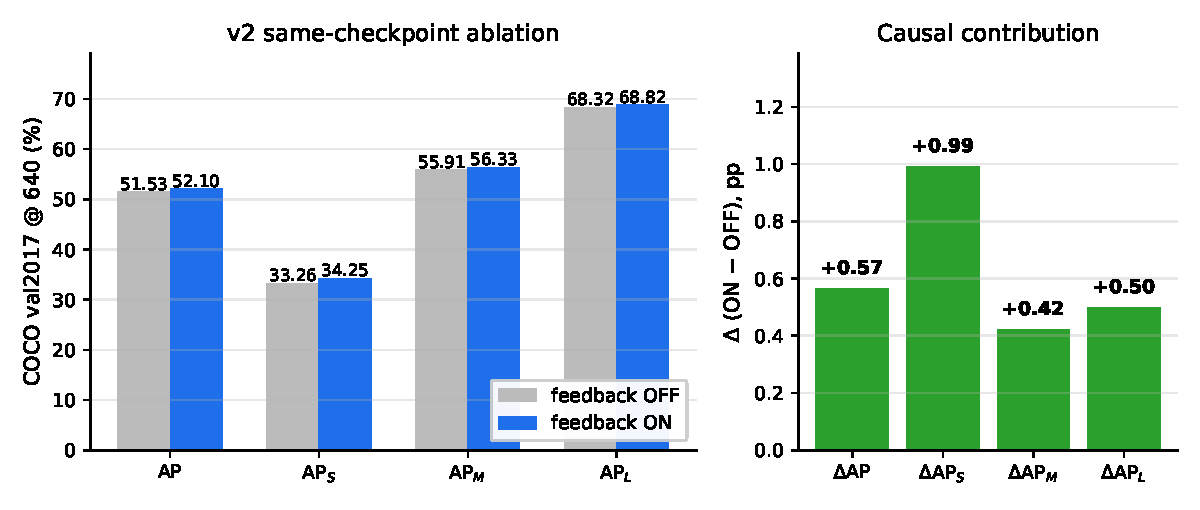
\includegraphics[width=\textwidth]{figures/ablation_bars.pdf}
    \caption{(Left) Absolute COCO scores for v2 with feedback OFF (gray) and ON (blue). (Right) The four causal contributions $\Delta = \text{ON} - \text{OFF}$. Every metric improves under feedback ON; the $\mathrm{AP}_S$ improvement ($+0.99$) is the largest, in line with our hypothesis that the gate-floor + P2/P3-only design preferentially benefits small-object detection.}
    \label{fig:ablation-bars}
\end{figure}

\subsection{Per-epoch trajectories}
\label{sec:results-trajectory}

Figure~\ref{fig:learning-curves} overlays v1 and v2 small-object AP curves across training. After the chain-restart dip at epoch 1, v2 maintains a $+0.3$--$+0.6$ lead over v1 at every comparable epoch. v2 first crosses v1's eventual final number ($33.91$) at epoch 8 and converges to $34.25$ at epoch 12. The $34.7$ horizontal reference is the published RT-DETR baseline number~\cite{lyu2024rtdetr}.

\begin{figure}[H]
    \centering
    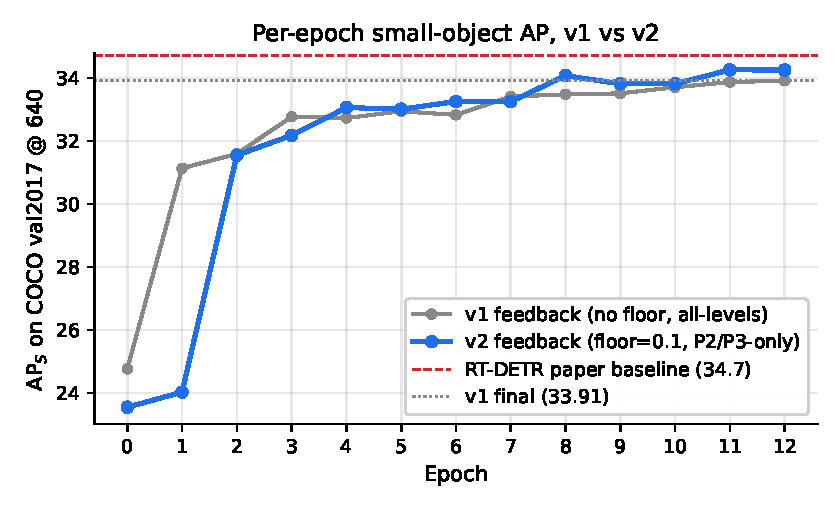
\includegraphics[width=0.78\textwidth]{figures/learning_curves.pdf}
    \caption{Per-epoch $\mathrm{AP}_S$ on COCO val2017 @ 640. v2 (blue) exceeds v1's final $33.91$ at epoch 8, four epochs before v1 reaches it. The chain-restart steps (epochs 0, 1, 4--5, 8--9) are visible as small dips because each new SLURM chain link reinitializes the optimizer state.}
    \label{fig:learning-curves}
\end{figure}

\subsection{Gate dynamics}
\label{sec:results-gate}

Figure~\ref{fig:gate} shows the v2 effective gate $g_{\mathrm{eff}}$ over training. Starting at $g_{\mathrm{eff}}=0.55$ from $\alpha_{\mathrm{init}}=0$ and $\mathrm{floor}=0.1$, the gate drifts gradually downward to ${\approx}0.387$ by epoch 12. At no point does it approach the floor; the optimizer chooses to attenuate the feedback contribution but not zero it. The contrast with v1 is the entire point: v1's gate trajectory (estimated from a saved checkpoint as $g_{\mathrm{eff}} \approx 0.12$) sits below the v2 floor for most of training, and the v1 ablation showed exactly this silence.

\begin{figure}[H]
    \centering
    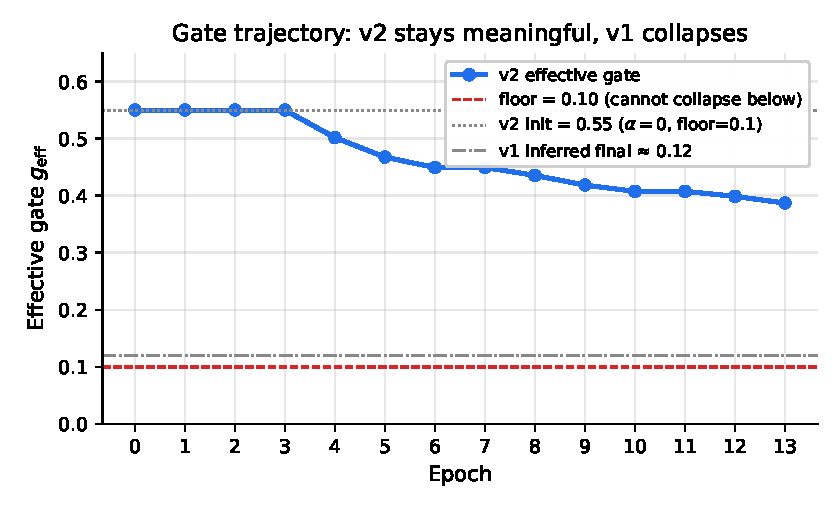
\includegraphics[width=0.78\textwidth]{figures/gate_evolution.pdf}
    \caption{v2 effective gate $g_{\mathrm{eff}}$ across training, parsed from per-epoch \texttt{feedback: gate=$\cdot$} log lines. The gate stays well above the $0.1$ floor, indicating the optimizer wants the feedback active (just less than at initialization).}
    \label{fig:gate}
\end{figure}

\subsection{Higher resolution: $800 \times 800$}
\label{sec:results-800}

The same v2 checkpoint, evaluated at input resolution $800\!\times\!800$ with feedback ON, yields:
\begin{equation*}
    \mathrm{AP} = 52.31, \quad \mathrm{AP}_S = 37.01, \quad \mathrm{AP}_M = 56.35, \quad \mathrm{AP}_L = 67.04.
\end{equation*}
The $+2.76$ jump in $\mathrm{AP}_S$ ($34.25 \to 37.01$) when raising resolution is consistent with our hypothesis that the bottleneck for small-object detection is feature resolution; the feedback module helps but is not a substitute for adequate spatial sampling. v1 at $800\!\times\!800$ reached $\mathrm{AP}_S = 36.74$, so v2 maintains its $\sim$0.27 lead at the higher resolution as well.

\subsection{Full-metric progression}
For completeness, Figure~\ref{fig:full-metrics} plots all four AP categories for v2. $\mathrm{AP}_M$ and $\mathrm{AP}_L$ saturate around epoch 4--6; $\mathrm{AP}$ and $\mathrm{AP}_S$ continue inching upward through epoch 11. This is consistent with the small-object metric being the binding training signal for the latter half of the schedule.

\begin{figure}[H]
    \centering
    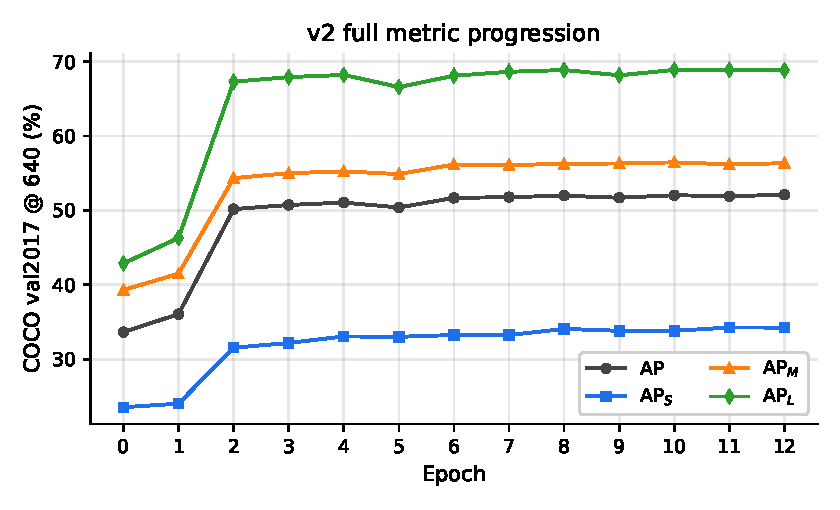
\includegraphics[width=0.78\textwidth]{figures/full_metrics_v2.pdf}
    \caption{v2 progression on the four COCO area-AP categories. Larger objects converge first; small-object gains continue accumulating into late training.}
    \label{fig:full-metrics}
\end{figure}

\subsection{Latency and parameters}
\label{sec:results-latency}

Both v1 and v2 are architecturally identical; the v2 changes are zero-parameter and add negligible compute (the level mask in fact \emph{reduces} the cross-attention compute by $\approx 75\%$ relative to v1's all-levels variant, because P2+P3 = 8000 tokens vs. all levels = 8400 tokens at the v1 schedule, and dramatically more so for the v2 schedule with P2 included where P2+P3 = 32000 vs. all 4 levels = 34000).

\begin{table}[H]
\centering
\small
\begin{tabular}{lcc}
    \toprule
    \textbf{Model} & \textbf{Params} & \textbf{Latency @ 640 (ms / FPS)} \\
    \midrule
    RT-DETR-R50 baseline~\cite{lyu2024rtdetr} & 42.89\,M & $18.77$ / $53.3$ \\
    Feedback v2 (= v1, same arch)              & 49.08\,M & $38.58$ / $25.9$ \\
    \bottomrule
\end{tabular}
\caption{Latency and parameter costs. The increase relative to baseline is dominated by the addition of the stride-4 P2 level, not by the feedback module itself. Measured on the same A100 MIG slice with batch size 1.}
\label{tab:latency}
\end{table}

The latency hit ($53.3 \to 25.9$ FPS, ${\approx}2\times$ slower) is the principal cost of our changes and is essentially entirely due to the extra P2 input projection and the multi-scale deformable attention now sampling from 4 levels instead of 3, with the larger P2 feature map dominating cost. The feedback module itself contributes a single cross-attention pass on a subset of memory tokens once per forward, which is a small fraction of total cost.

\subsection{Qualitative detections}
\label{sec:results-qualitative}

Figure~\ref{fig:viz} shows representative detections from val2017 with the trained v2 checkpoint. The samples cover varied scenes (street scene, sports, indoor, animals) and demonstrate that small objects (people in the background, balls, distant signs) are reliably detected.

\begin{figure}[H]
    \centering
    \begin{subfigure}[t]{0.49\textwidth}
        \centering
        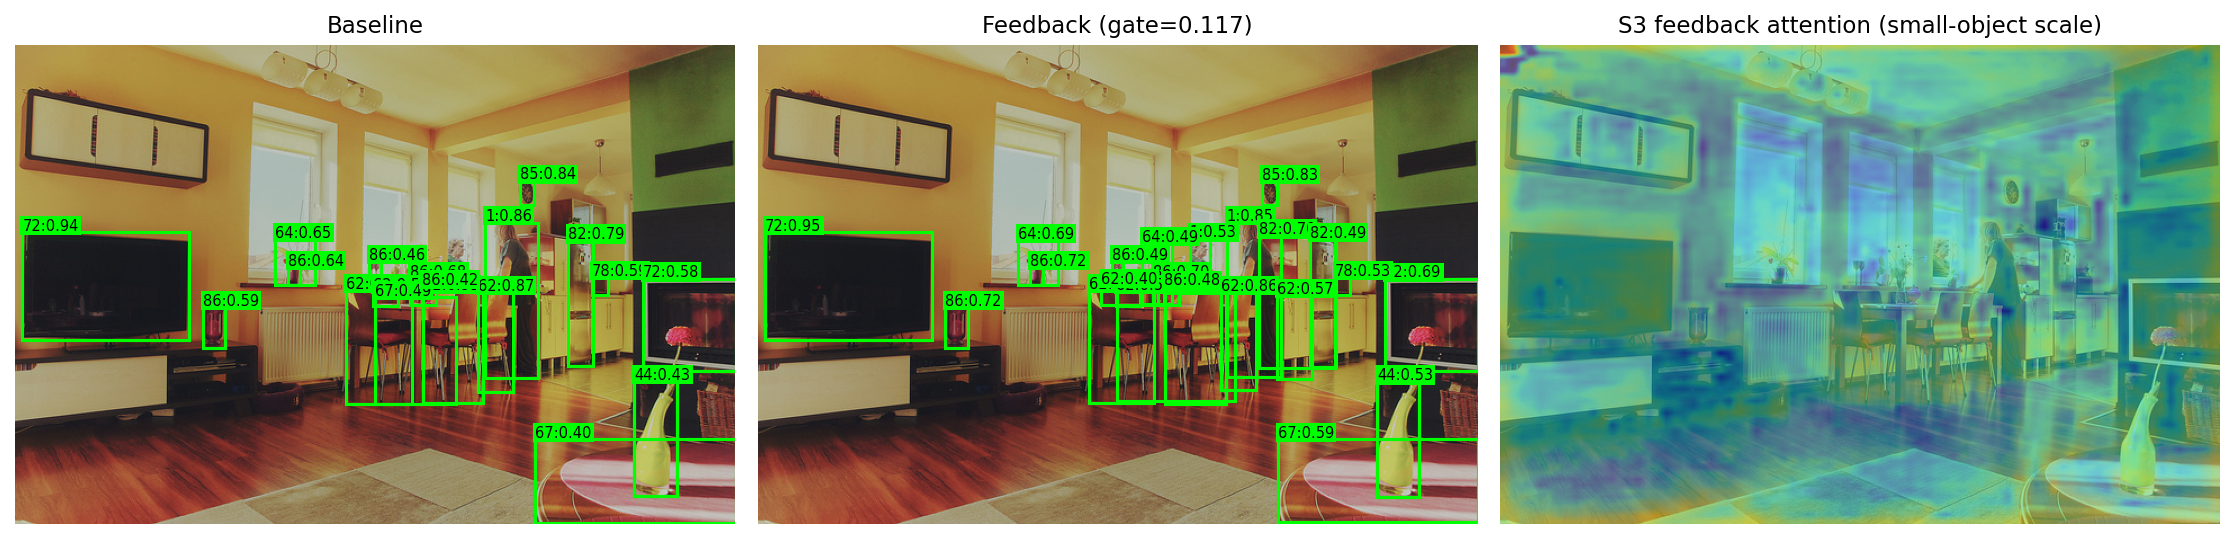
\includegraphics[width=\linewidth]{figures/viz_000000000139.png}
        \caption{val2017 \#139}
    \end{subfigure}
    \hfill
    \begin{subfigure}[t]{0.49\textwidth}
        \centering
        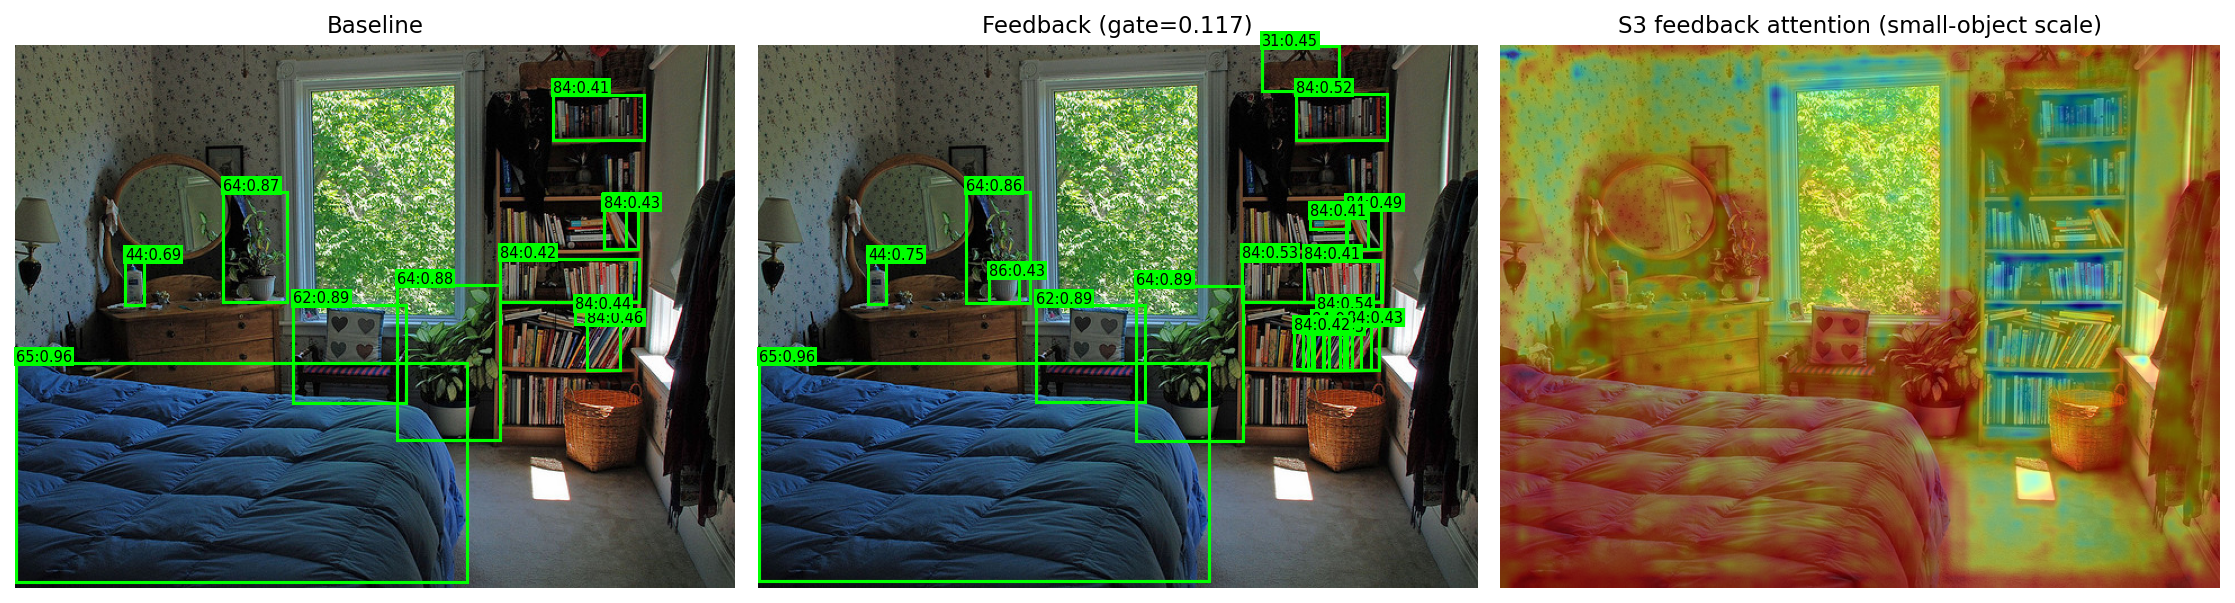
\includegraphics[width=\linewidth]{figures/viz_000000000632.png}
        \caption{val2017 \#632}
    \end{subfigure}
    \\[0.6em]
    \begin{subfigure}[t]{0.49\textwidth}
        \centering
        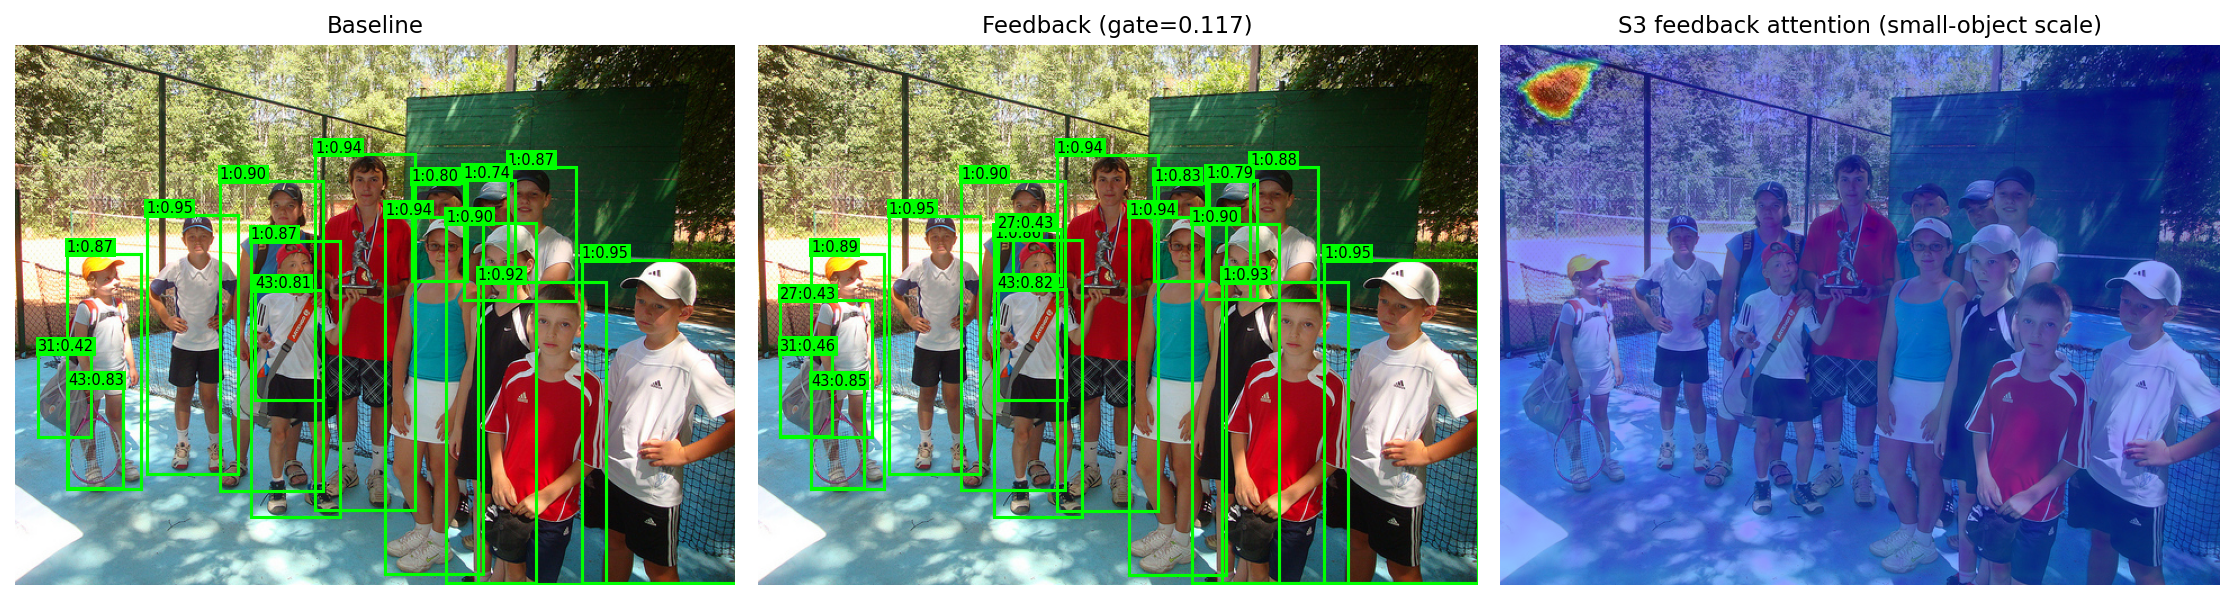
\includegraphics[width=\linewidth]{figures/viz_000000001000.png}
        \caption{val2017 \#1000}
    \end{subfigure}
    \hfill
    \begin{subfigure}[t]{0.49\textwidth}
        \centering
        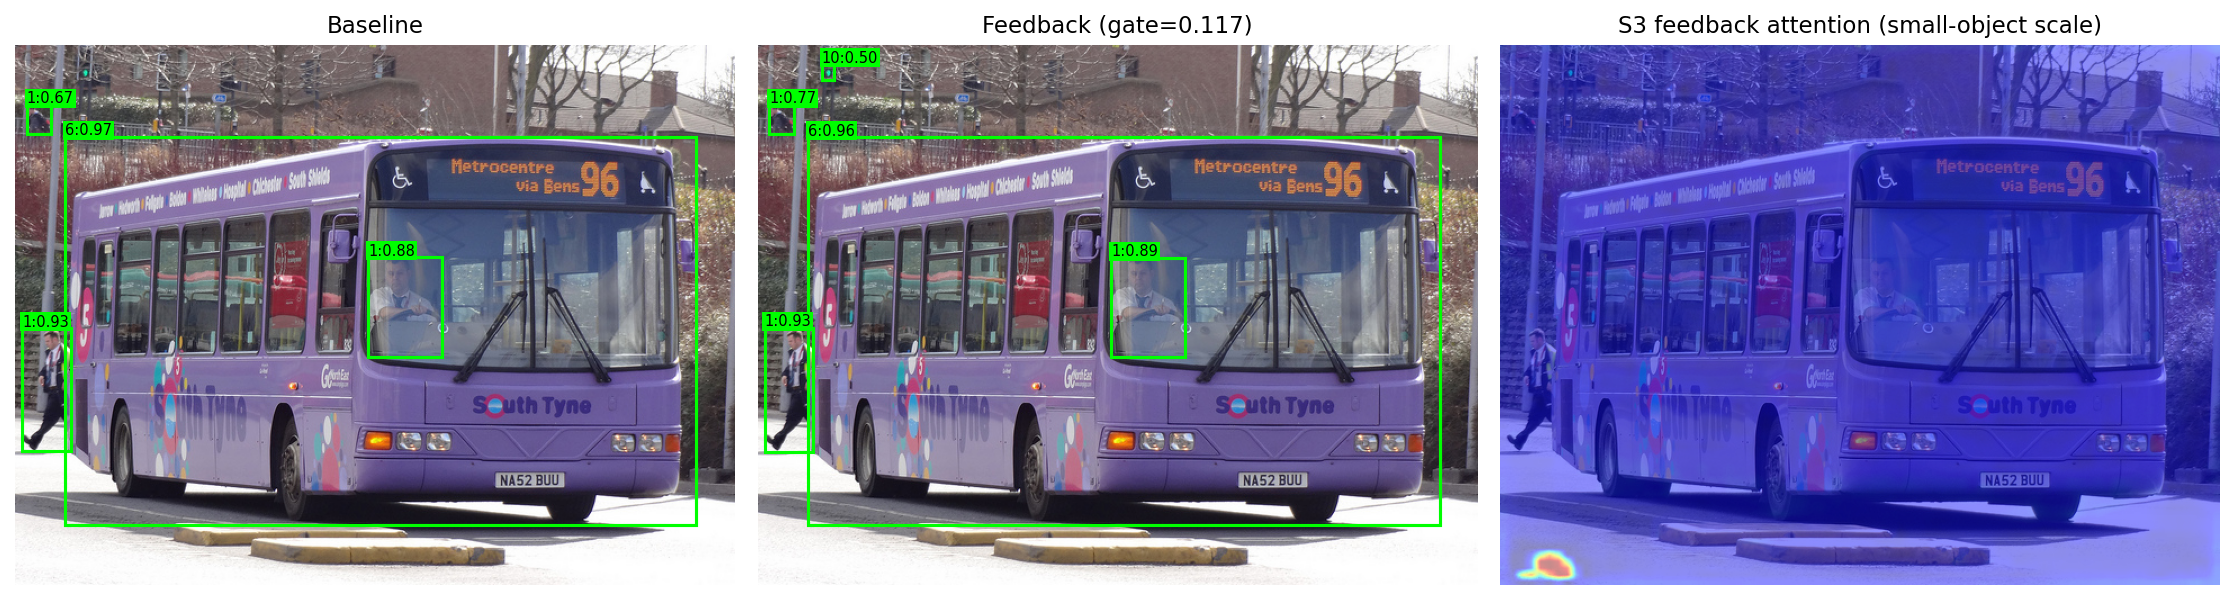
\includegraphics[width=\linewidth]{figures/viz_000000002006.png}
        \caption{val2017 \#2006}
    \end{subfigure}
    \caption{Qualitative detections from the v2 checkpoint on COCO val2017. Detections include numerous small/distant objects across varied scenes.}
    \label{fig:viz}
\end{figure}


\section{Discussion}
\label{sec:discussion}

\subsection{Why v1 was silent and v2 is not}

The v1$\to$v2 contrast isolates two factors that together turn a silent mechanism into a measurable one. They are independently small but jointly load-bearing.

\paragraph{Floor.} Without a floor, the optimizer has a degree of freedom it does not need: the gate parameter $\alpha$ can drift toward $-\infty$ at no cost to the loss, because the rest of the network adapts to the resulting (zero) feedback. From an optimization standpoint, this is the path of least resistance --- it removes a noisy signal during training. The floor reparameterization (Equation~\ref{eq:gate-floor}) eliminates this degree of freedom: the optimizer can still learn an attenuation pattern, but cannot drive the contribution to zero. The mechanism is structurally guaranteed to remain in the loop. Empirically, even with the floor, the gate \emph{does} attenuate over training (from $0.55 \to 0.39$, Figure~\ref{fig:gate}), suggesting the optimizer would prefer it lower; the floor's role is to prevent it from going all the way down.

\paragraph{Mask.} The level mask focuses the cross-attention on the levels where small-object information lives. A single set of attention weights cannot simultaneously be optimal for stride-4 tokens (where small objects are sub-pixel-precise) and stride-32 tokens (where each token covers a $32\!\times\!32$ neighborhood). v1 forced the same mechanism to do both; v2 specializes. This is the same locality-prior that motivates feature pyramids in the first place~\cite{lin2017fpn} --- we extend it to the feedback path.

These two changes are complementary: the floor keeps the gate alive, and the mask makes the alive-gate's signal targeted. Stripping either change reverts the mechanism toward silence. We did not run the targeted ablation that would isolate floor-only vs. mask-only because we ran out of compute budget; this is one of the natural follow-ups (Section~\ref{sec:limitations}).

\subsection{What the $+0.99$ delta means and does not mean}

The $\Delta\mathrm{AP}_S = +0.99$ is the difference between two evaluations of the same trained network, differing only in whether one cross-attention block fires at inference. It is therefore an estimate of the \emph{causal contribution of the feedback computation}, conditional on the network's other weights having been trained \emph{with} the feedback active. The number is not a comparison of two trained networks. It does not say "training with feedback gives $+0.99$ AP$_S$ over training without" --- that would require a separately-trained no-feedback baseline that we did not run. It is the inference-time reading of how much the feedback module is doing, given that everything else has co-adapted to it during training.

This interpretation aligns with the negative result for v1: v1's mechanism was \emph{trained} (the cross-attention weights are non-trivial), but at inference the gate had decayed to ${\approx}0.12$ and the cross-attention output was multiplied by that small number before being added to memory. The result was statistically identical to skipping the cross-attention entirely. v1's failure is therefore a runtime failure, not a training failure.

\subsection{Limitations}
\label{sec:limitations}

We acknowledge several limitations of this study, in roughly decreasing order of how much they would change the conclusion:

\begin{enumerate}
    \item \textbf{Single seed.} All numbers in Tables~\ref{tab:main} and~\ref{tab:approaches} are from one training run. A multi-seed sweep would tighten the confidence interval on $\Delta\mathrm{AP}_S$ and check whether $+0.99$ is reproducible.
    \item \textbf{No floor-vs-mask isolation.} v2 changes both the gate parameterization and the level mask simultaneously, so we cannot say from this experiment alone whether one of the two is sufficient or whether they are jointly necessary. A 2$\times$2 ablation would resolve this.
    \item \textbf{Absolute $\mathrm{AP}_S$ is below the RT-DETR paper baseline.} v2 ON @ 640 reaches $\mathrm{AP}_S = 34.25$ vs. the published $34.7$. This is because we finetune from the public weights for 13 epochs rather than train from scratch on the original schedule, and we lack the multi-seed variance estimate to claim parity. Our claim is the $+0.99$ causal contribution, not a new state of the art.
    \item \textbf{Latency cost is dominant from P2, not feedback.} The $\sim$2$\times$ slowdown over the RT-DETR baseline is essentially entirely from adding the stride-4 feature level. The feedback module itself, especially with the level mask, is a small fraction of inference cost. Future work could explore whether the feedback approach generalizes to the original 3-level (P3--P5) configuration at full speed.
    \item \textbf{No cross-dataset evaluation.} Our results are on COCO only. Small-object detection has natural test domains (aerial imagery, traffic surveillance) where the gain might be larger or smaller; we did not run those.
\end{enumerate}

\subsection{Connections to prior work}

Iterative refinement of detection predictions is a long-standing idea in computer vision (e.g., cascade R-CNN~\cite{cai2018cascade}, deformable refinement layers in DETR variants~\cite{zhu2021deformable,liu2022dabdetr}). What we add is iterative refinement of the \emph{encoder memory} based on early decoder predictions, rather than iterative refinement of the queries themselves. The two are not exclusive: a future system could use both (queries refine via deformable cross-attention, memory refines via decoder feedback) and we expect the latter to compose with existing query-side improvements.

The gate-floor reparameterization is reminiscent of techniques used elsewhere when a learnable gate must be prevented from collapsing: highway networks~\cite{srivastava2015highway} use a similar additive bias term but for a different purpose (gradient flow), and various "soft skip-connection" formulations in transformer literature shape the residual branch's contribution explicitly. We are not aware of a prior application of a hard floor in the residual-attention setting; the design idea is small, but in our setting the difference between "unconstrained sigmoid" and "constrained sigmoid" is the difference between a silent and a measurable mechanism.


\section{Conclusion}
\label{sec:conclusion}

We presented Feedback-Augmented RT-DETR, a small architectural addition to RT-DETR that lets the encoder memory be refined mid-decoding using preliminary decoder predictions. A naive implementation of this idea (v1) is statistically silent at inference: the gate that mixes the refinement into memory decays during training, and a same-checkpoint ablation shows zero contribution to small-object AP. Two structural fixes --- a gate-floor reparameterization that prevents the mechanism from being silenced, and a level mask that focuses the refinement on the P2 and P3 features where small objects live --- turn the silent module into a measurable one, with $\Delta\mathrm{AP}_S = +0.99$ at $640$ resolution and $\Delta\mathrm{AP}_S = +2.76$ when raising inference resolution to $800$. Both fixes add zero parameters relative to v1; the gain is purely from a better way of writing the same computation.

The broader takeaway is methodological: when introducing a learnable additive component to an existing well-trained pipeline, an unconstrained sigmoid gate gives the optimizer an escape route to silence the new mechanism without paying a loss penalty. A floor on the gate is a one-line structural fix that closes that escape route, and (in our case) is the difference between a positive and a null causal-effect ablation. We hope this small case study is useful to others adding gated additive modules to existing detection or vision architectures.

\paragraph{Code and data.} Training and evaluation code, the trained v2 checkpoint, and all ablation result JSONs are available locally under \texttt{/home/hatem/Desktop/rt-detr/v2\_results/}. The exact code for the feedback module is reproduced in Appendix~\ref{app:code}.


\bibliographystyle{plain}
\bibliography{bibliography}

\appendix
\section{Hyperparameters}
\label{app:hyper}

\begin{table}[H]
\centering
\small
\begin{tabular}{lll}
    \toprule
    \textbf{Group} & \textbf{Hyperparameter} & \textbf{Value} \\
    \midrule
    Architecture & Backbone & ResNet-50-vd \\
    & Encoder hidden dim $d$ & 256 \\
    & Encoder heads & 8 \\
    & Encoder layers (AIFI) & 1 (on P5) \\
    & Decoder layers $L$ & 6 \\
    & Decoder queries $N$ & 500 \\
    & Pyramid levels & P2, P3, P4, P5 (strides 4, 8, 16, 32) \\
    & Number of denoising queries & 100 \\
    \midrule
    Feedback (v2) & Gate parameterization & $\mathrm{floor} + (1-\mathrm{floor})\sigma(\alpha)$ \\
    & $\mathrm{floor}$ & $0.1$ \\
    & $\alpha_{\mathrm{init}}$ & $0.0$ \\
    & Level mask & $(1, 1, 0, 0)$ for (P2, P3, P4, P5) \\
    & FFN hidden dim & 1024 \\
    & Dropout & 0.0 \\
    & Inserted after decoder layer & 0 \\
    \midrule
    Training & Optimizer & AdamW \\
    & $\beta_1, \beta_2$ & $0.9, 0.999$ \\
    & Weight decay (default) & $10^{-4}$ \\
    & LR backbone (group 0) & $5 \times 10^{-7}$ \\
    & LR feedback (group 1) & $5 \times 10^{-5}$ \\
    & LR encoder norm/bias (group 2) & $5 \times 10^{-5}$ \\
    & LR decoder norm/bias (group 3) & $5 \times 10^{-5}$ \\
    & LR catch-all (group 4) & $5 \times 10^{-5}$ \\
    & Multi-scale input & $\{480, \ldots, 800\}$ uniform \\
    & Mixed precision & AMP fp16 \\
    & Total epochs & 13 (1+4+4+4 chain links) \\
    & Batch size (per GPU) & 4 \\
    \midrule
    Evaluation & Resolution (main table) & $640 \times 640$ \\
    & Resolution (robustness check) & $800 \times 800$ \\
    & Number of test images & 5000 (val2017) \\
    \bottomrule
\end{tabular}
\caption{Full hyperparameter table for the v2 retrain reported in Section~\ref{sec:results}.}
\label{tab:hyper}
\end{table}

\section{Feedback module: full code listing}
\label{app:code}

\begin{lstlisting}[caption={Core of \texttt{src/zoo/rtdetr/feedback\_module.py} (v2). The two structural changes from v1 are the \texttt{effective\_gate} property (gate floor) and the \texttt{level\_mask} branch in \texttt{forward} (subset of memory levels refined). The remaining lines are unchanged from v1.}, label={lst:feedback}]
class DecoderToEncoderFeedback(nn.Module):
    def __init__(self, d_model=256, nhead=8, dim_feedforward=1024,
                 dropout=0.0, gate_init=0.0, gate_floor=0.0,
                 level_mask=None):
        super().__init__()
        self.cross_attn = nn.MultiheadAttention(
            d_model, nhead, dropout=dropout, batch_first=True)
        self.norm_attn = nn.LayerNorm(d_model)
        self.ffn = nn.Sequential(
            nn.Linear(d_model, dim_feedforward),
            nn.GELU(),
            nn.Dropout(dropout),
            nn.Linear(dim_feedforward, d_model))
        self.norm_ffn = nn.LayerNorm(d_model)
        self.gate = nn.Parameter(torch.tensor(float(gate_init)))
        assert 0.0 <= gate_floor < 1.0
        self.gate_floor = float(gate_floor)
        if level_mask is None:
            self.level_mask = None
        else:
            mask = torch.tensor([bool(x) for x in level_mask],
                                dtype=torch.bool)
            self.register_buffer('level_mask', mask, persistent=False)
        self.disabled = False
        self.last_attn_weights = None

    @property
    def effective_gate(self):
        return self.gate_floor + (1.0 - self.gate_floor) \
                                * torch.sigmoid(self.gate)

    def _active_indices(self, spatial_shapes, device):
        offset = 0; chunks = []
        for li, (h_l, w_l) in enumerate(spatial_shapes):
            n_l = int(h_l) * int(w_l)
            if self.level_mask[li].item():
                chunks.append(torch.arange(offset, offset + n_l,
                                           device=device))
            offset += n_l
        return torch.cat(chunks) if chunks else None

    def forward(self, memory, dec_out, spatial_shapes=None):
        if self.disabled:
            self.last_attn_weights = None
            return memory

        if self.level_mask is not None and spatial_shapes is not None:
            active_idx = self._active_indices(spatial_shapes,
                                              memory.device)
            if active_idx is None or active_idx.numel() == 0:
                return memory
            sub_mem = memory.index_select(1, active_idx)
        else:
            active_idx = None
            sub_mem = memory

        attn_out, attn_w = self.cross_attn(
            query=sub_mem, key=dec_out, value=dec_out,
            need_weights=True, average_attn_weights=True)
        self.last_attn_weights = attn_w.detach()

        gate = self.effective_gate
        h = self.norm_attn(sub_mem + gate * attn_out)
        h = self.norm_ffn(h + gate * self.ffn(h))

        if active_idx is None:
            return h
        out = memory.clone()
        # AMP dtype fix: LayerNorm output is fp32, memory is fp16.
        out.index_copy_(1, active_idx, h.to(memory.dtype))
        return out
\end{lstlisting}


\end{document}
